%!TEX root = foo-thesis.tex

\chapter{Concept}

\section{Global Illumination Pipeline Overview}
\label{sec:concept:overview}

\begin{figure}[h]
    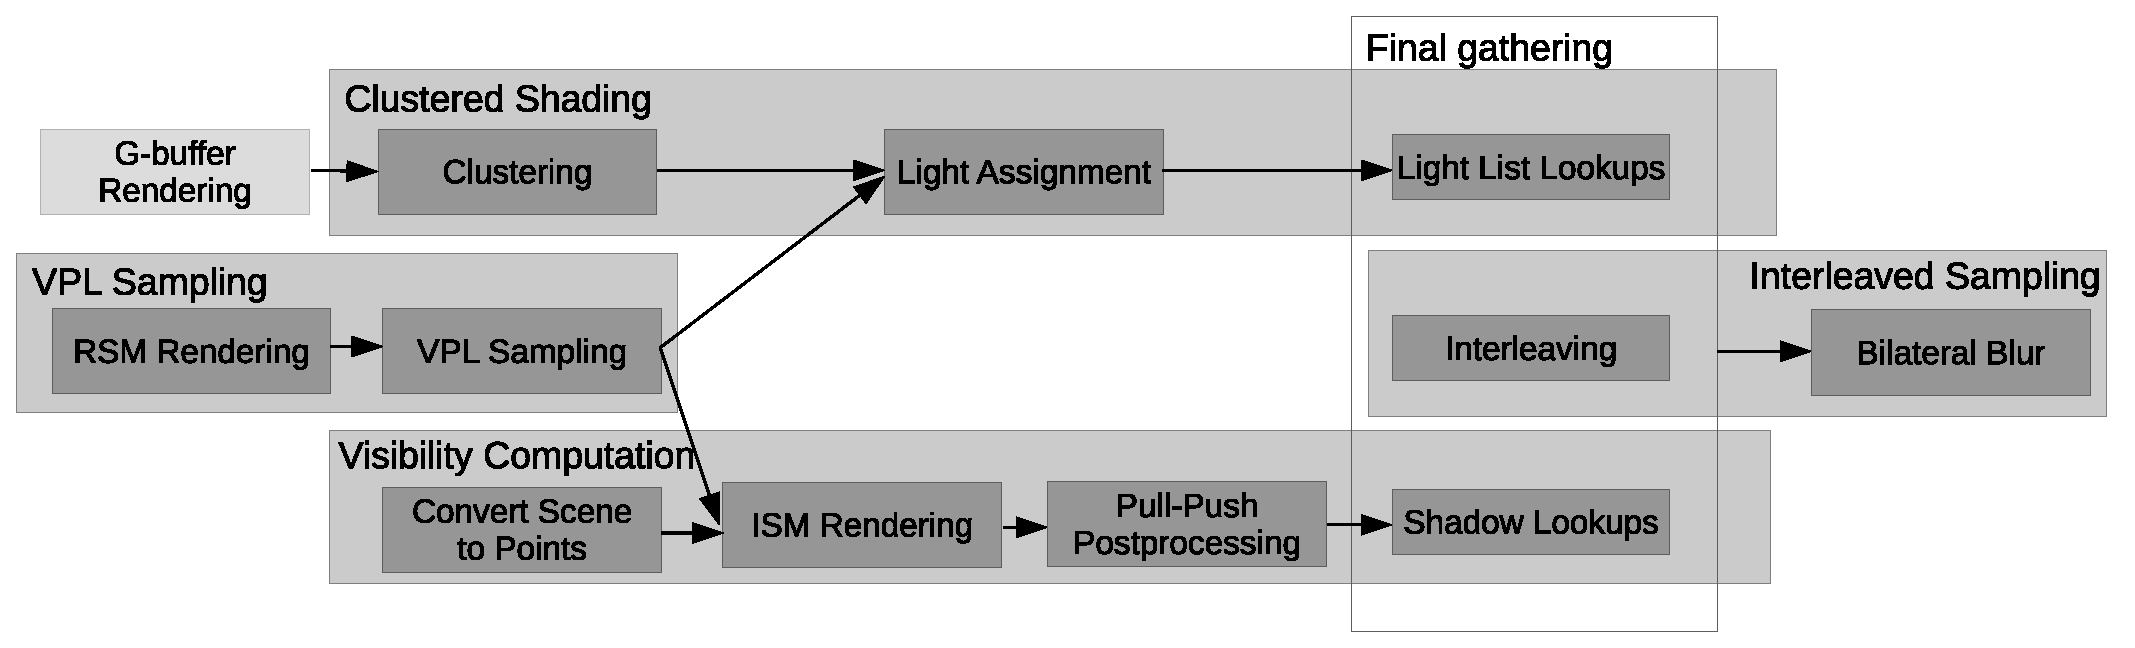
\includegraphics[width=\textwidth]{graphics/GI_pipeline_concept_rough}
    \caption{Global Illumination pipeline concept.}
    \label{fig:GIPipelineConcept}
\end{figure}


This chapter will detail the individual stages of the global illumination pipeline presented in this thesis. Figure~\ref{fig:GIPipelineConcept} provides an overview.
The reflective shadow map and the subsequent VPL sampling (left part of middle row in the diagram) will be covered in the following section.
Section~\ref{sec:concept:ism} describes the rendering process for the imperfect shadow maps (lower row) in detail.
The final gathering step uses data from the clustered shading technique (upper row, detailed in Section~\ref{sec:concept:clusteredShading}) and performs interleaved sampling (right part of middle row, detailed in Section~\ref{sec:interleavedSampling}.
Our G-buffer rendering does not differ from common deferred rendering pipelines and is not covered further.
Finally, we use clamping to remove singularities, this is shortly presented in Section~\ref{sec:concept:clamping}.


\section{Virtual Point Light Sampling with Reflective Shadow Maps}
\label{sec:concept:rsmVplSampling}

VPL sampling has not been the focus of this thesis, therefore we use a rather basic approach by rendering a  reflective shadow map \parencite{Dachsbacher:2005:RSM} and regularly sampling it. \citet{hedman2016sequential} present a more advanced approach.

\begin{outline}
\1 Often preferred due to the simplicity and speed because rasterization. but, first bounce only.

\1 Similar to regular G-Buffer rendering

\1 Like shadowmaps, scene is rendered from the light's viewpoint

\1 Unlike shadowmaps, not only depth is rendered but additionally normal and (diffuse) surface color.

\1 The result can be sampled to create VPLs with a certain position reconstructed from the depth buffer, and normal and color taken from the additional buffers.

\1 In our case, we use regular sampling. Importance-based approaches are available, also the samples can be clustered \cite{} or chosen relative to their estimated contribution to the final output. \citet{hedman2016sequential} uses a different approach without RSMs.

\end{outline}

\section{Visibility Computation with Imperfect Shadow Maps}
\label{sec:concept:ism}


The original paper \citep{ritschel2008ism} converts the scene geometry to a point set in a preprocessing step and uses the points to efficiently render hundreds of shadow maps in parallel. They use splatting to render the points and fill the resulting holes in the shadowmaps with a pull-push algorithm inspired by \citep{Marroquim:2007:reconstruction}.

\citet{ritschel2011ismsViewAdaptive} build on this by converting the scene to a triangle texture dynamically, and sampling the points from that texture. Instead of computing a triangle texture, \citet{barak2013temporally} use the tessellation units of recent GPUs to dynamically convert triangles into points.
We follow this approach since it is relatively simple to implement and inherently dynamic, but have not implemented the adaptive sampling from \citet{ritschel2011ismsViewAdaptive} yet.
\citet{ritschel2008ism} also present multi-bounce indirect illumination with their technique, which we have not implemented.
We describe the point rendering process in the following section and subsequently detail the pull-push algorithm.

\subsection{Point Rendering with Splatting}
\begin{outline}
\1 render the scene
\1 depending on the size of the triangle, set tessellation levels
\1 of the resulting tessellated triangles, take the center, calculate approx world size of disk, take normal from buffer
\1 while it might be faster to just use the vertices as points, we take the center of each triangle to be more accurate, otherwise the points on the edge of the triangle will enlarge the rendered area considerably.
\1 pick a random VPL, perform culling, render splat into the VPL's ISM. To simplify the calculations, the ISM uses a paraboloid mapping. Here another advantage of the points comes into play: Compared to triangles it is trivial to perform a paraboloid projection for points.
\1 As an optimization, we iterate over several VPLS, and collect some that pass the culling test, and render to those. more in implementation chapter
\1 To remove holes in the resulting shadowmap, the original paper implements a simplified variant of \citet{Marroquim:2007:reconstruction} that only uses depth information from the point rendering. We found that this approach has little benefit over simply enlarging all the point splats during rendering, therefore we did not use it when using splat rendering.
\end{outline}

\subsection{Point Rendering with Pull-Push Postprocessing}

\begin{outline}
\1 Besides point splat rendering, we also persued a second approach that follows the approach of \citet{Marroquim:2007:reconstruction} more closely. More specifically points are rendered as a single pixel, albeit with additional attributes like size and normal. These are then used in a subsequent reconstruction pass to create an (ideally) hole-free shadowmap.

\1 rough overview: the algorithm is a ``pyramid-method'' and uses miplevels.
\1 a pull phase aggregates the information from four pixels of a finer level to one pixel of a coarser level.
\1 It only considers valid pixels, i.\,e. ???
\1 the push phase aggregates four pixels of the coarser level for each pixel of the finer level.
\1 Again only pixels that are valid, i.\,e. ???
\1 we differ from the original implementation by...
\end{outline}
\todo{expand on this}



\section{Clustered Deferred Shading}
\label{sec:concept:clusteredShading}


\begin{outline}
\1 in addition to interleaved sampling, we also employ a technique taken from \citet{olsson2012clustered}
\1 view frustum is divided into a fixed number of clusters
\1 for each fragment, determine cluster. clusters with no fragments are ignored.
\1 for each cluster, determine the VPLs that can reach that cluster, put into light list.
\1 during shading, don't iterate over all VPLs but only those from the light list.
\1 usually, large benefits due to limited radius. we have infinite radius, but at least we can discard half the lights because hemisphere.
\todo{ritschel's paper about clustering}
\end{outline}




\section{Interleaved Sampling}
\label{sec:concept:interleavedSampling}
Interleaved sampling \citep{Keller:2001:InterleavedSampling} is often used to vastly improve the performance impact of GI methods.

\begin{outline}
\1 general idea: given some amount of samples that, in a naïve implementation, would be performed per pixel, distribute those samples over a 4x4 or 8x8 block of pixel
\1 the naïve implementation hurts cache coherency, since adjacent pixels process different samples.
\1 to this end, de-interleaving \citep{segovia2006non} is often used to simultaneously process those pixels that use the same sample set. see Section~\ref{sec:impl:interleavedShading} for details.

\1 results in structured noise and missing information as all pixels have only part of the samples
\1 therefore, geometry-aware blur similar to \citet{laine2007incremental} to distribute the information

\1 all this works because low-frequency effect

\1 In most aspects we follow this standard approach. The only notable deviation is our implementation of de-interleaving that does not use any separate splitting/merging passes, again we defer details to Section~\ref{sec:impl:interleavedShading}.

\end{outline}



\section{Removing Lighting Singularities through Clamping}
\label{sec:concept:clamping}
It's simple, we clamp the singularities. Wouldn't be necessary with infinite number of lights. \citet{hedman2016sequential} reach high accuracy even with clamping and 2k lights.
